\documentclass{article}
\usepackage{fullpage}
\usepackage{amsmath}
\usepackage{amssymb}
\usepackage{graphicx}
\usepackage{url, hyperref}

\renewcommand{\Pr}[1]{\mathbb{P}\left[#1\right]}
\newcommand{\Ex}[1]{\mathbb{E}\left[#1\right]}
\newcommand{\Var}[1]{\text{Var}\left[#1\right]}

\renewcommand{\bf}[1]{\mathbf{#1}}
\newcommand{\bs}[1]{\boldsymbol{#1}}
\newcommand{\mat}[1]{\ensuremath{\begin{pmatrix} #1 \end{pmatrix}}}

\title{\large CS480/680, Spring 2023\\\huge Assignment 1}

\author{Designer: Haochen Sun; Instructor: Hongyang Zhang}
\date{Released: May 15; Due: June 4, noon}
\setlength\parindent{0pt}

\begin{document}

\maketitle

\subsection*{Instructions}

\begin{itemize}
    \item We do not accept hand-written submissions.
    \item This assignment is due by noon on June 4, 2023.
    \item For questions labelled as ``\textbf{coding}'', please follow the instructions provided and implement the required features. The \href{https://colab.research.google.com/gist/jvhs0706/3f0778cc9fbbf4a077f752ea1edf956b/cs480-680-assignment1-coding.ipynb}{skeleton code} is provided. Unless otherwise specified, all implementations should be in \emph{Python} using a \emph{Jupyter Notebook}. Before submission, please make sure that your code can run without any errors. Also, be sure to save the output of each cell, as any missing output may not be graded.
    \item Please submit the following TWO files to LEARN:
    \begin{itemize}
        \item A write-up in PDF format: the written answers to ALL questions, including the reported results and plots of coding questions, in a single PDF file.
        \item An IPYNB file: your implementations for ALL coding questions. Please save the output of each cell, or your coding questions may NOT be graded.
    \end{itemize}
\end{itemize}

\newpage
\subsection*{Question 1: Perceptron (30 points)}

\begin{enumerate}
    \item \textbf{[15 points]} Consider the AND, OR and XOR datasets, each of which labels all two-dimensional binary inputs $\left\{\mat{0\\0}, \mat{0\\1}, \mat{1\\0}, \mat{1\\1}\right\}$:

    \begin{table}[h]
        \centering
        \begin{tabular}{c|cccc}
             ~ & \mat{0\\0} & \mat{0\\1} & \mat{1\\0} & \mat{1\\1} \\
             \hline
             AND & 0 & 0 & 0 & 1 \\
             OR & 0 & 1 & 1 & 1 \\
             XOR & 0 & 1 & 1 & 0
             
             
        \end{tabular}
        \caption{The AND, OR and XOR datasets}
        \label{tab:xor}
    \end{table} 

    For each dataset, prove or disprove if it is linearly separable. For a linearly separable dataset, write down the separating hyperplane. For a non-linearly separable dataset, argue that a separating hyperplane does not exist.

    Solution: 

    For AND dataset, it is linearly separable, and one of the separating hyper planes is $$\omega =\mat{1\\1}$$ and $$b=-1.5$$

    For OR dataset, it is linearly separable, and one of the separating hyper planes is $$\omega = \mat{1\\1}$$ and $$b=-0.5$$

    For XOR dataset, it is not linearly separable, and the following is the proof:

    Suppose the dataset is separable, thus there exist $\omega$ and $b$ such that for all points, $sign(<x,\omega >+b)$ matches the data.
    
    Note that $$\mat{1\\0} + \mat{0\\1} = \mat{1\\1}$$ so we have that there exists $\omega$ and $b$ such that
    $$<\mat{1\\0},\omega >+b + <\mat{0\\1},\omega >+b = <\mat{1\\1},\omega >+b$$

    But, from data set, the sign of RHS should be different from the sign of LHS. Which is a contradiction.

    Therefore, XOR dataset is not linearly separable.

    \item \textbf{[15 points, coding]} Implement the \href{https://hongyanz.github.io/slides/cs480680_s23_Lecture2.pdf#page=13}{perceptron algorithm} on the \href{https://archive.ics.uci.edu/ml/datasets/spambase}{Spambase dataset} in \emph{Python} using \emph{Jupyter Notebook}. You may use the provided \href{https://colab.research.google.com/gist/jvhs0706/3f0778cc9fbbf4a077f752ea1edf956b/cs480-680-assignment1-coding.ipynb}{skeleton code}, which downloads and pre-processes the dataset. Note that the target variable to be predicted is the last feature, \texttt{is\_spam}. Plot the accuracy against the number of training steps and report the final accuracy.
    \begin{figure}
        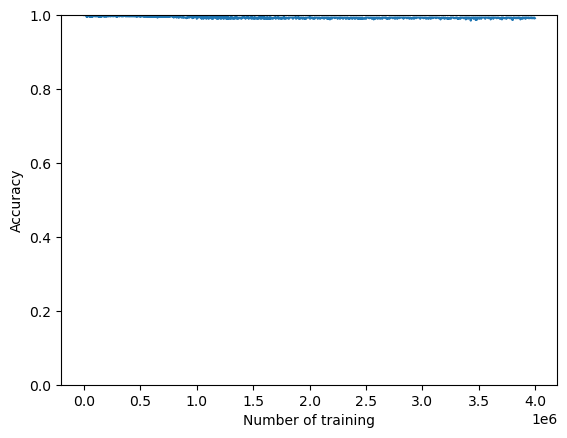
\includegraphics[width=\linewidth]{IMG.png}
    \end{figure}

    It seems that the final accuracy is fluctuated around 1.
\end{enumerate}


\newpage
\subsection*{Question 2: Generalized Linear Models (40 points)}
In class, we have discussed linear regression and logistic regression. While these models are useful for specific types of data, they belong to a broader class of models known as generalized linear models (GLMs). GLMs are models for data where the response variable $y$ follows a distribution from the exponential family, and the mean of the response variable is related to the predictors via a link function. The GLM has the following form:

\begin{equation} \label{eq:glm-def}
p(y|\mathbf{x}, \mathbf{w}, \tau) = h(y, \tau)\exp\left[\frac{y\eta-A(\eta)}{d(\tau)}\right],
\end{equation}

where $p$ is the probability mass function or probability density function of $y$, $\eta := \mathbf{w}^\top\mathbf{x}$ is the natural parameter, $A(\eta)$ is the log normalizer, and $\tau$ is the dispersion parameter, such that $d(\tau)>0$ typically related to the variance of the conditional distribution. $h(y, \tau)$ is a normalization factor such that $p(y|\bf{x}, \bf{w}, \tau)$ sums/integrates to $1$ over $y$. We denote the mapping from the linear input $\eta = \mathbf{w}^\top\mathbf{x}$ to the conditional expectation of $y$ (i.e., $\mu = \mathbb{E}[y|\mathbf{x}, \mathbf{w}, \tau]$) as $\mu = \ell^{-1}(\eta)$, where $\ell$ is known as the link function, and $\ell^{-1}$ is known as the mean function. (For simplicity, omit the bias term throughout this question.) %The link function determines how the predictors are related to the mean of the response variable. In linear regression, the link function is the identity function, while in logistic regression, it is the logit function. In the following questions, we will explore some properties of GLMs and their applications.

\begin{enumerate}
    \item \textbf{[10 points]} Show that linear regression and logistic regression are special cases of the GLM in \eqref{eq:glm-def}. Identify $h(y,\tau)$, $A(\eta)$, $d(\tau)$, and the link function $\ell$ for each case. %(\textbf{Hint}: For linear regression, assume that $y \sim \mathcal{N}(\mu, \sigma^2)$, and show that this distribution belongs to the exponential family. For logistic regression, assume that $y \sim \text{Ber}(p)$, where $p = \sigma(\mu)$, and show that this distribution belongs to the exponential family. Then, identify the relevant parameters $h(y,\tau)$, $A(\eta)$, $d(\tau)$, and $\ell$ for each case.)% (Hint: treat $\tau$ as the variance $\sigma^2$ in the linear regression case).
    \begin{itemize}
        \item Comparing the probability mass function of linear regression to the GLM, it is easy to notice that $h(y,\tau)=\frac{1}{\sqrt{2\pi \sigma^2}}$ and $\frac{y\eta-A(\eta)}{d(\tau)}=-\frac{1}{2\sigma^2}(y-\eta)^2$
        \item Comparing the later equation, also notice that $d(\tau) > 0$, we have $d(\tau)=2\sigma^2$, $A(\eta)=y^2+\eta^2-y\eta$. Notice that $\tau=\sigma^2$, we then have $h(y,\tau)=\frac{1}{\sqrt{2\pi\tau}}$, $d(\tau)=2\tau$.
        \item Rearrange the form of logistic regression, we have 
        \item $p(y|x,w)=\frac{(e^{-\eta})^{1-y}}{1+e^{-\eta}}=\frac{e^{-\eta}}{(1+e^{-\eta})e^{-y\eta}}=\frac{1}{1+e^{-\eta}}exp(y\eta - \eta)$
        \item By comparing, we get $h(y,\tau)=\frac{1}{e^{-\eta}}$, $A(\eta)=\eta$, and $d(\tau)=1$.
    \end{itemize}
    \item \label{poisson} \textbf{[6 points]} Consider the Poisson regression model, which is defined by the following probability mass function: \[p(y|\mathbf{x},\mathbf{w})=\text{Pois}(y|\exp(\mathbf{w}^\top\mathbf{x})).\]Here, $\text{Pois}(y|\mu)=\frac{\mu^ye^{-\mu}}{y!}$ is the Poisson distribution parameterized by $\mu$, with support $y\in\mathbb{N}$. Show that Poisson regression belongs to the family of GLMs defined in Equation \eqref{eq:glm-def}, and identify $A(\eta)$ for this model.
    \begin{itemize}
        \item Rearrange the expression, we have $p(y|x,w)=\frac{e^{y\eta} e^{-e^\eta}}{y!}=\frac{1}{y!}exp(y\eta - e^y)$
        \item Then by comparing, we have $A(\eta)=e^y$
    \end{itemize}
    \item \label{nll} \textbf{[8 points]} Consider a dataset $\left\{\left(\mathbf{x}_n,y_n\right)\right\}_{n=1}^N$, where $\mathbf{x}_n\in\mathbb{R}^d$ and $y_n$ is the response variable. Derive the negative log-likelihood (NLL) for the GLM on this dataset based on Equation \eqref{eq:glm-def}. Explain how the derived NLL is equivalent to the square loss (for linear regression) and binary cross entropy loss (for logistic regression) for finding the optimal $\bf{w}$.
    \begin{itemize}
        \item $-log(P(y|x,w,\tau))=-log(h(y,\tau)exp(\frac{y\eta-A(\eta)}{d(\tau)}))=-log(h(y,\tau))-\frac{y\eta-A(\eta)}{d(\tau)}$
    \end{itemize}
    \item \textbf{[6 points]} Derive the negative log-likelihood (NLL) loss function for the Poisson regression model using the results from sub-questions \ref{poisson} and \ref{nll}. Simplify the expression as much as possible.
    \begin{itemize}
        \item From 2, we have $A(\eta)=e^y$, $d(\tau)=1$, $h(y,\tau)=\frac{1}{y!}$
        \item Sub these into the form we have in 3, we get the NLL is $-log(\frac{1}{y!})-y\eta+e^y$
    \end{itemize}
    \item \textbf{[10 points]} Prove that in Equation \eqref{eq:glm-def}, $\Ex{y|\bf{x}, \bf{w}, \tau} = A'(\eta)$ and $\Var{y|\bf{x}, \bf{w}, \tau} = A''(\eta)d(\tau)$. (Hint: you may either assume that $y$ is discrete or continuous. As the first step, sum/integrate both sides of Equation \eqref{eq:glm-def} over $y$. You may switch the order of the summation/integration and the derivative without justification.)
    \begin{itemize}
        \item Assume it is continuous.
        \item $\int{h(y,\tau)exp[\frac{y\eta - A(\eta)}{d(\tau)}] dy}$
    \end{itemize}
\end{enumerate}

\newpage
\subsection*{Question 3: SVM kernels (30 points)}
\begin{enumerate}
    \item \textbf{[10 points]} Given a natural number $M$, consider $X = \{0, 1, \dots M\}$. Define $K (x, x') = \min\{x, x'\}$. Find a mapping $\phi: X \to \mathbb{R}^M$ such that for all $x, x'\in X$, $K(x, x') = \left\langle \phi(x), \phi(x')\right\rangle$.
    \begin{itemize}
        \item Assume $\phi(x)=(\phi_1(x),\phi_2(x),...,\phi_M(x))$
        \item Then $<\phi(x),\phi(x')>=\sum_{i=1}^{M}{\phi_i(xx')}$
    \end{itemize}
    \item \textbf{[10 points]} Show that there exists a Hilbert space $H$ and a mapping $\phi: \mathbb{R}^n\to H$ such that \[\left\langle \phi(\bf{u}), \phi(\bf{v})\right\rangle = 4\left\langle \bf{u}, \bf{v}\right\rangle^2 + \left\langle \bf{u}, \bf{v}\right\rangle^3\] for all $\bf{u}, \bf{v}\in \mathbb{R}^n$. (Hint: consider $H = \mathbb{R}^{n^2 + n^3}$.)
    \begin{itemize}
        \item Let $\phi(x)=((x\bigotimes x\bigotimes x,x\bigotimes x))$
        \item Then
        \begin{math}
            <\phi(u),\phi(v)> = <(u\bigotimes u\bigotimes u,u\bigotimes u),(v\bigotimes v\bigotimes v,v\bigotimes v)>\\
            = <u\bigotimes u\bigotimes u,v\bigotimes v\bigotimes v>+<u\bigotimes u, v\bigotimes v> \\
            =<u\bigotimes u\bigotimes u,v\bigotimes v\bigotimes v> + \sum_{i}\sum_{j}{u_iu_jv_iv_j}=<u\bigotimes u\bigotimes u,v\bigotimes v\bigotimes v>+(\sum{u_iv_i})^2
        \end{math}
    \end{itemize}
    \item \textbf{[10 points]} More generally, consider a polynomial $f$ with non-negative coefficients, and construct $H$ and $\phi$ such that \[\left\langle \phi(\bf{u}), \phi(\bf{v})\right\rangle= f(\left\langle \bf{u}, \bf{v}\right\rangle)\] for all $\bf{u}, \bf{v} \in \mathbb{R}^n$. 
    \begin{itemize}
        \item Let $f=\sum{a_ix^i}$
        \item Define $\phi(x)=(\sqrt{a_0}x_0, \sqrt{a_1}x_1, ... ,\sqrt{a_{n-1}}x_{n-1})$, note that $\phi: \mathbb{R}^n \to \mathbb{R}^n$
        \item Then we have 
        \begin{math}
            <\phi(u),\phi(v)>=<(\sqrt{a_0}u_0, \sqrt{a_1}u_1, ... ,\sqrt{a_{n-1}}u_{n-1}), (\sqrt{a_0}v_0, \sqrt{a_1}v_1, ... ,\sqrt{a_{n-1}}v_{n-1})> \\
            =a_0u_0v_0 + a_1u_1v_1 + ... + a_{n-1}u_{n-1}v_{n-1} = f(<u,v>)
        \end{math}
    \end{itemize}
\end{enumerate}

\end{document}
